\chapter{対象とするゲーム}
\section{はじめに} 
システムの有用性を検証するために、今回はこのシステムの利用に想定されうるサンプルゲームを実装した。

この章では、このゲームのルールや、採用理由について解説し、このゲーム固有のシステムの設計について述べる。

\section{ゲームの概要} 
\subsection{基本ルール} 
今回、対象としたゲームは、ターン型完全情報のパズルゲームである。
このゲームは、10x10の盤面を操作し、キャラクターがゴール状態に辿り着くまでに繰り返す。
プレイヤーは一人でプレイする
\subsection{ターンの流れ}
まず、プレイヤーは盤面の中から隣接する2x2の任意の4マスについて選択する。

\begin{figure}[htbp]
  \begin{center}
    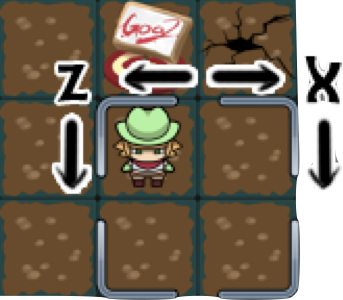
\includegraphics[bb=0 0 172 150, width=4cm]{images/41.png}
  \end{center}
  \caption{初期状態}
  \label{fig:one}
\end{figure}

選択したマスについて、プレイヤーは選択したマスを右方向、ないしは左方向に回転させる。
ただし、何も無い空白のマスを含む4マスは回転させることができない。
マップを回転させると、上に乗っているオブジェクトやキャラクターも同様のルールによって回転する。(図4-2)

\begin{figure}[htbp]
  \begin{center}
    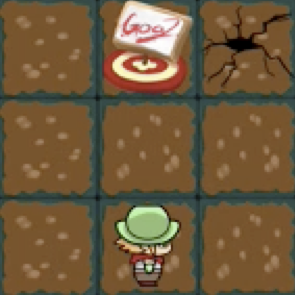
\includegraphics[bb=0 0 172 150, width=4cm]{images/42.png}
  \end{center}
  \caption{プレイヤー操作後の状態}
  \label{fig:one}
\end{figure}

次に、プレイヤーキャラクターは、現在向いている方向に自動的に移動する。移動はスキップすることができない。(図4-3)

\begin{figure}[htbp]
  \begin{center}
    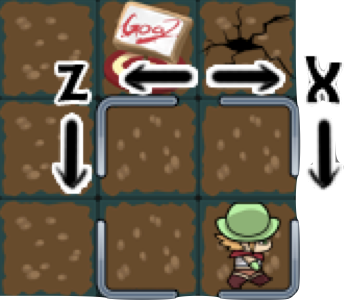
\includegraphics[bb=0 0 172 150, width=4cm]{images/43.png}
  \end{center}
  \caption{ターン終了時の状態}
  \label{fig:one}
\end{figure}

この一連の2つのステップを1ターンと定義する。プレイヤーはターンを終了状態に到達するまで繰り返し、
これを1ゲームとする。
\subsection{ゲームの終了条件}
ターンを繰り返し、いずれかの状態になったとき、1ゲームが終了する。

\subsubsection{クリア条件}
以下の状態になったとき、そのゲームはクリア状態となる
\begin{itemize}
  \item プレイヤーキャラクターがゴールマスに到達したとき
\end{itemize}

\subsubsection{ゲームオーバー条件}
以下の状態になったとき、そのゲームは失敗となり、ゲームオーバーになる
\begin{itemize}
    \item プレイヤーキャラクターがマップ外にはみ出したとき
    \item 死亡判定のあるギミックに触れたとき(穴や針など)
\end{itemize}

\subsection{マップ上のギミック}
マップ上のギミックとして、下記の物が実装されている。

\subsubsection{岩}
キャラクターは進入することができず、進行方向逆向きに方向を転換し、1マス進む。
進むべき方向に別の岩がある場合、方向のみを切り替える。

\begin{figure}[htbp]
  \begin{center}
    
\includegraphics[bb=0 0 24 24, width=2.5cm]{images/rock.png}
  \end{center}
  \caption{岩}
  \label{fig:one}
\end{figure}

\subsubsection{穴}
プレイヤーキャラクターが進入するとゲームオーバーとなる。プレイヤー以外のキャラクターが進入すると消滅する。

\begin{figure}[htbp]
  \begin{center}
    
\includegraphics[bb=0 0 24 24, width=2.5cm]{images/hole.png}
  \end{center}
  \caption{穴}
  \label{fig:one}
\end{figure}

\subsubsection{針}
キャラクターが4方向のうち、針の向いている方向から進入すると、穴と同様でゲームオーバーになる。
針のないその他の3方向から進入したとき、岩と同様の扱いとなる。

\begin{figure}[htbp]
  \begin{center}
    
\includegraphics[bb=0 0 24 24, width=2.5cm]{images/needle.png}
  \end{center}
  \caption{針}
  \label{fig:one}
\end{figure}

\subsubsection{滑る床}
プレイヤーキャラクターが進入すると、自動的に向いている方向にもう1マス進む。
進んだ後に進入した床がさら滑る床だった場合、
再帰的に進み続ける。

\begin{figure}[htbp]
  \begin{center}
    
\includegraphics[bb=0 0 24 24, width=2.5cm]{images/ice.png}
  \end{center}
  \caption{滑る床}
  \label{fig:one}
\end{figure}

\subsubsection{崩れる床}
1度目の進入は通常の床として扱う。崩れる床から他のマスに移動したとき、崩れる床は穴に変化する。以降は穴として扱う。

\begin{figure}[htbp]
  \begin{center}
    
\includegraphics[bb=0 0 24 24, width=2.5cm]{images/broken.png}
  \end{center}
  \caption{崩れる床}
  \label{fig:one}
\end{figure}

\section{対象ゲームの採用目的}
このゲームをシステムの適応として採用したのは、以下の理由が挙げられる。
\subsubsection{操作が容易でプレイヤー間の実力差が出にくいため}
ルールさえ習得できれば、複雑な操作が必要なく、マウスのみで遊べるため、非常にプレイしやすい。
特殊な操作も必要のないため、先行研究で利用されていた『Infinite Mario』などに比べ、誰もが上達しやすいため。
\subsubsection{確定完全情報ゲームであるため}
ランダム性が一切ないため。ランダム要素を含むゲームだと、収集したログの解析が難しい物になってしまう。
また、ある手を取ったとき、次の状態が確定するため、計算機上でのシミュレーションも容易であるため、ログを収集した
データの定量的評価が行いやすい。
\subsubsection{リプレイ性が高いため}
様々な手を試し、試行錯誤をはかるゲームであるため、リプレイ性が高いと予想できる。
そのため、プレイ回数に応じたプレイヤー力量の変化を観測しやすい。

\subsubsection{問題空間が小さく、解の探索が容易なため}
プレイヤーの取れる行動が非常に少ないため、計算機上での全探索による解の探索、ソルバーの実装が容易である。

\subsubsection{レベル作成が非常に困難を極めるため}
レベルデータの作成は人の手によって行われているが、良質なレベルの作成が非常に困難である。
そのため、収集したプレイヤーログをレベル作成に生かすことができれば、非常に有用な物となるため。


\section{対象ゲームの解の探索}
プレイヤーが取れる入力の総数Xは以下の数式で表される

\[ X = (2((W-1)・(H-1)))^T \]

ただし、W マップの横幅 H マップの高さ、Tは総ターン数

しかし、実際は何も無いマスを含む回転は行えないため、回転カ所は非常に限定される。

\section{対象ゲームに特化したシステム設計}
対象ゲームにおいて、前章において述べたそれぞれのモデルは、以下のようなデータ構造で記述できる

\subsection{Level}
各「レベル」を定義するLevelモデルは以下の情報を保持すれば良いと考えられる

\paragraph{map}
マップ情報を定義する二次元配列を文字列としてJSON形式で格納している。ゲーム実行時にクライアント側でパースし、ステージとして読み込む

例えば、以下の図のようなマップは、このようなテキストデータを格納することにより、記述している。

\begin{figure}[htbp]
  \begin{center}
    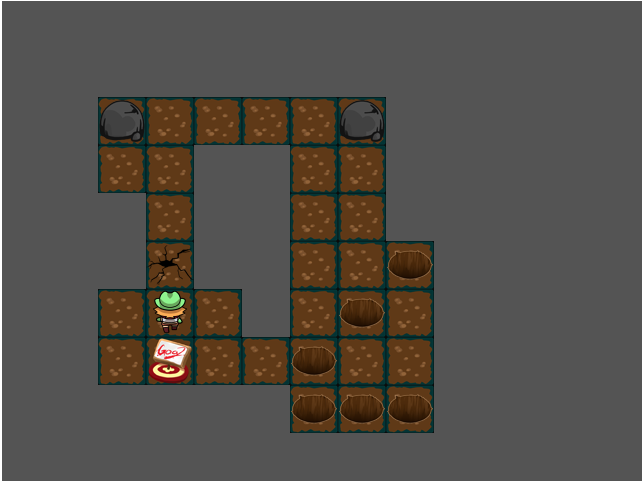
\includegraphics[bb=0 0  643 482, width=10cm]{images/json.png}
  \end{center}
  \caption{Levelデータの例}
  \label{fig:one}
\end{figure}

\begin{verbatim}
{``player'': [``3'', ``6'', 1], 
 ``map'': [
  [0, 0, 0, 0, 0, 0, 0, 0, 0, 0], 
  [0, 0, 0, 0, 0, 0, 0, 0, 0, 0], 
  [0, 0, 3, 1, 0, 0, 1, 1, 0, 0], 
  [0, 0, 1, 1, 1, 5, 1, 2, 0, 0], 
  [0, 0, 1, 0, 0, 0, 1, 1, 0, 0], 
  [0, 0, 1, 0, 0, 0, 0, 1, 0, 0], 
  [0, 0, 1, 1, 1, 1, 1, 4, 4, 0], 
  [0, 0, 3, 1, 1, 1, 4, 1, 4, 0], 
  [0, 0, 0, 0, 0, 4, 1, 1, 4, 0], 
  [0, 0, 0, 0, 0, 0, 0, 0, 0, 0]
 ]
}
\end{verbatim}
playerはプレイヤーの初期座標と方向、mapはLevel上の配置データを行列で保持している。
この行列は、実際に表示されているマップデータとは異なり、転置されていることに留意されたい。

\subsection{Operation}
プレイヤーの行動を定義するOperationモデルは以下の情報を保持すれば良いと考えられる

\paragraph{x}
回転する4マスのうち、左上のマスのx座標が記録される
\paragraph{y}
回転する4マスのうち、左上のマスのy座標が記録される
\paragraph{direction}
回転方向が0または1で記録される
\paragraph{timestamp}
Operationが発行された日時がミリ秒単位で記録される

このゲームにおいては、このOperationを保存しておくことで、プレイヤーの動きを完全に再現できる。
